\documentclass[]{article}
\usepackage{ listings} 
\usepackage{graphicx}
\graphicspath{ {images/} }
\usepackage{float}
\usepackage{geometry}
\usepackage{pdfpages}
\usepackage{multirow}

\usepackage{algorithm}  
\usepackage{algpseudocode}  
\usepackage{amsmath} 

\renewcommand{\algorithmicrequire}{\textbf{Input:}}
\renewcommand{\algorithmicensure}{\textbf{Output:}}

\makeatletter
\def\@maketitle{%       
	\newpage
	\null
	\vskip 14em%
	\begin{center}%
		\let \footnote \thanks
		{\LARGE \@title \par}%
		\vskip 12em%
		{\large
			\lineskip .5em%
			\begin{tabular}[t]{c}%
				\@author
			\end{tabular}\par}%
		\vskip 1em%
		{\large \@date}%
	\end{center}%
	\par
	\vskip 1.5em}
\makeatother
%opening
\title{\Huge COT5405 - Analys of Algorithms \\ Homework 2}
\author{Qinxuan Shi \\ UFID: 83518162}
\date{}
\special{papersize=8.5in,11in}
\geometry{left=2cm,right=2cm,top=1.5cm,bottom=1.5cm}

\begin{document}
	
	\maketitle
	\clearpage
	
	\section{Problem 1: Weighted approximate common substring}
	\subsection{Pseudo-code of the Algorithm}
	\begin{algorithm}  
		\caption{Weighted approximate common substring}  
		\begin{algorithmic} 
			\Require String s1, String s2, dp[][]
			\Ensure
			\State We define that the best common substring means that the substring has the heaviest total weight.
			\State Assume that i is the rightmost index of the character in substring s1' of s1, and j is the rightmost index of the character in substring s2' of s2. And we define dp[i][j] to represent the weight of best common substring between s1' and s2'.
			\For{i= 0 to s1.length}
				\If{s2[0] exists in s1}
					\State dp[i][0] $\leftarrow$ $W_{s2[0]}$
				\Else
					\State dp[i][0] $\leftarrow$ 0
				\EndIf
			\EndFor
			
			\For{j= 0 to s2.length}
				\If{s1[0] exists in s2}
					\State dp[0][j] $\leftarrow$ $W_{s1[0]}$
				\Else
					\State dp[0][j] $\leftarrow$ 0
				\EndIf
			\EndFor
			
			\For{i= 0 to s1.length}
				\For{j= 0 to s2.length}
					\If{s1[i] = s2[j]}
						\State dp[i][j] $\leftarrow$ Maximum\_weight(i,j)
					\Else
						\State dp[i][j] $\leftarrow$ dp[i-1][j-1]
					\EndIf
				\EndFor
			\EndFor\\
			\Return max\{dp[i][j]\}.
		\end{algorithmic}  
	\end{algorithm} 

	\begin{algorithm}[H]  
		\caption{Maximum\_weight(i, j)}  
		\begin{algorithmic} 
			\Require String s1, String s2, int[] weight, int i, int j, dp[]
			\Ensure
			\State We now can get the substring s1' ended with index i and substring s2' ended with index j. Then we calculate the maximum subarray of them after transform them into weight int[] w.
			\If{t=0}
				\State dp[0] $\leftarrow$ w[0]
			\EndIf
			\For{i = 1 to w.length}
				\If{dp[i - 1] \textgreater 0}
					\State dp[i] $\leftarrow$ w[i] + dp[i - 1]
				\Else
					\State dp[i] $\leftarrow$ w[i]
				\EndIf
			\EndFor\\
			\Return max\{dp[i]\}
		\end{algorithmic}  
	\end{algorithm} 

	\subsection{Proof of the algorithm's correctness}
	
	Firstly, our goal is to get the best common substring. so we use OPT(i,j) to represent the best common substring s, i means the index of the rightmost character of s in the first string s1 and j means the index of the rightmost character of s in the second string s2.  \\ 
	
	\noindent Since when two characters are different, we have to minus $\delta$ to the total weight, it is clear that the best common substring has the property that $s1[i] = s2[j]$. Then, we are going to change the character into an array of weight with the length of $min\{s1(0,i).length, s2(0,j).length\}$ (because both substring of s1 and s2 are of the same length, the maximum length of the best common substring is the length of the shorter substring). \\            
	
	\noindent Bellman equation: \\
	
	OPT(i, j) =
	$\begin{cases} 
		Maximum\_weight(i, j),  & \mbox{if }\mbox{s1[i] = s2[j]} \\
		OPT(i-1, j-1), & \mbox{if }\mbox{s1[i] not euqal to s2[j]}
	\end{cases}$ \\
	
	\noindent Then, we are going to explain function Maximum\_weight. After transforming the english characters into numbers with the regulation which is starting from the last character of substring (index i in s1 and index j in s2), if these two characters of the substring s1' and substring s2' are the same, the character turns to the weight of the characher, while if the two characters are different, the number in the array of weight becomes -$\delta$.\\
	
	\noindent Now, we get the array of weight, and we are going to find the maximum sum of the array. Exactly, it's the same as the Maximum subarray problem. So we can deal with the problem with the following Bellman equation. \\
	
	Bellman equation\\
	
	OPT(i) =
	$\begin{cases} 
		x_{1},  & \mbox{if }\mbox{i = 1} \\
		max\{x_{i}, x_{i} + OPT(i-1)\}, & \mbox{if }\mbox{i \textgreater 1}
	\end{cases}$
	
	\subsection{Algorithm's running time}
	
	To the Algorithm Maximum\_weight, it is easy to get the complexity by using the KADANE’S algorithm, which is O(n). \\
	
	\noindent According to the pseudo-code, the first for-loop and the second for-loop are going to initialize the dp matrix which is used to memorize the maximum weight of each dp[i][j], so the complexity is O(n).  \\
	
	\noindent To the third for-loop, which is used to compute each dp[i][j], we assume that the length of s1 is M and the length of s2 is N, is the complexity of third for-loop is O(MN).It is also easy to know that if we want to find the maximum weight in the dp matrix, it takes O(MN).  \\
	
	\noindent To conclude, the total complexity of the algorithm is O(MN), which depends on the length of the two strings.  \\
	
	\noindent We could clearly infer from the result picture of 500 points of (MN, time) that $Time = k * MN$, so it is true for the proof that the total complexity of the algorithm is O(MN). \\
	
	\begin{figure}[H]
		\centering
		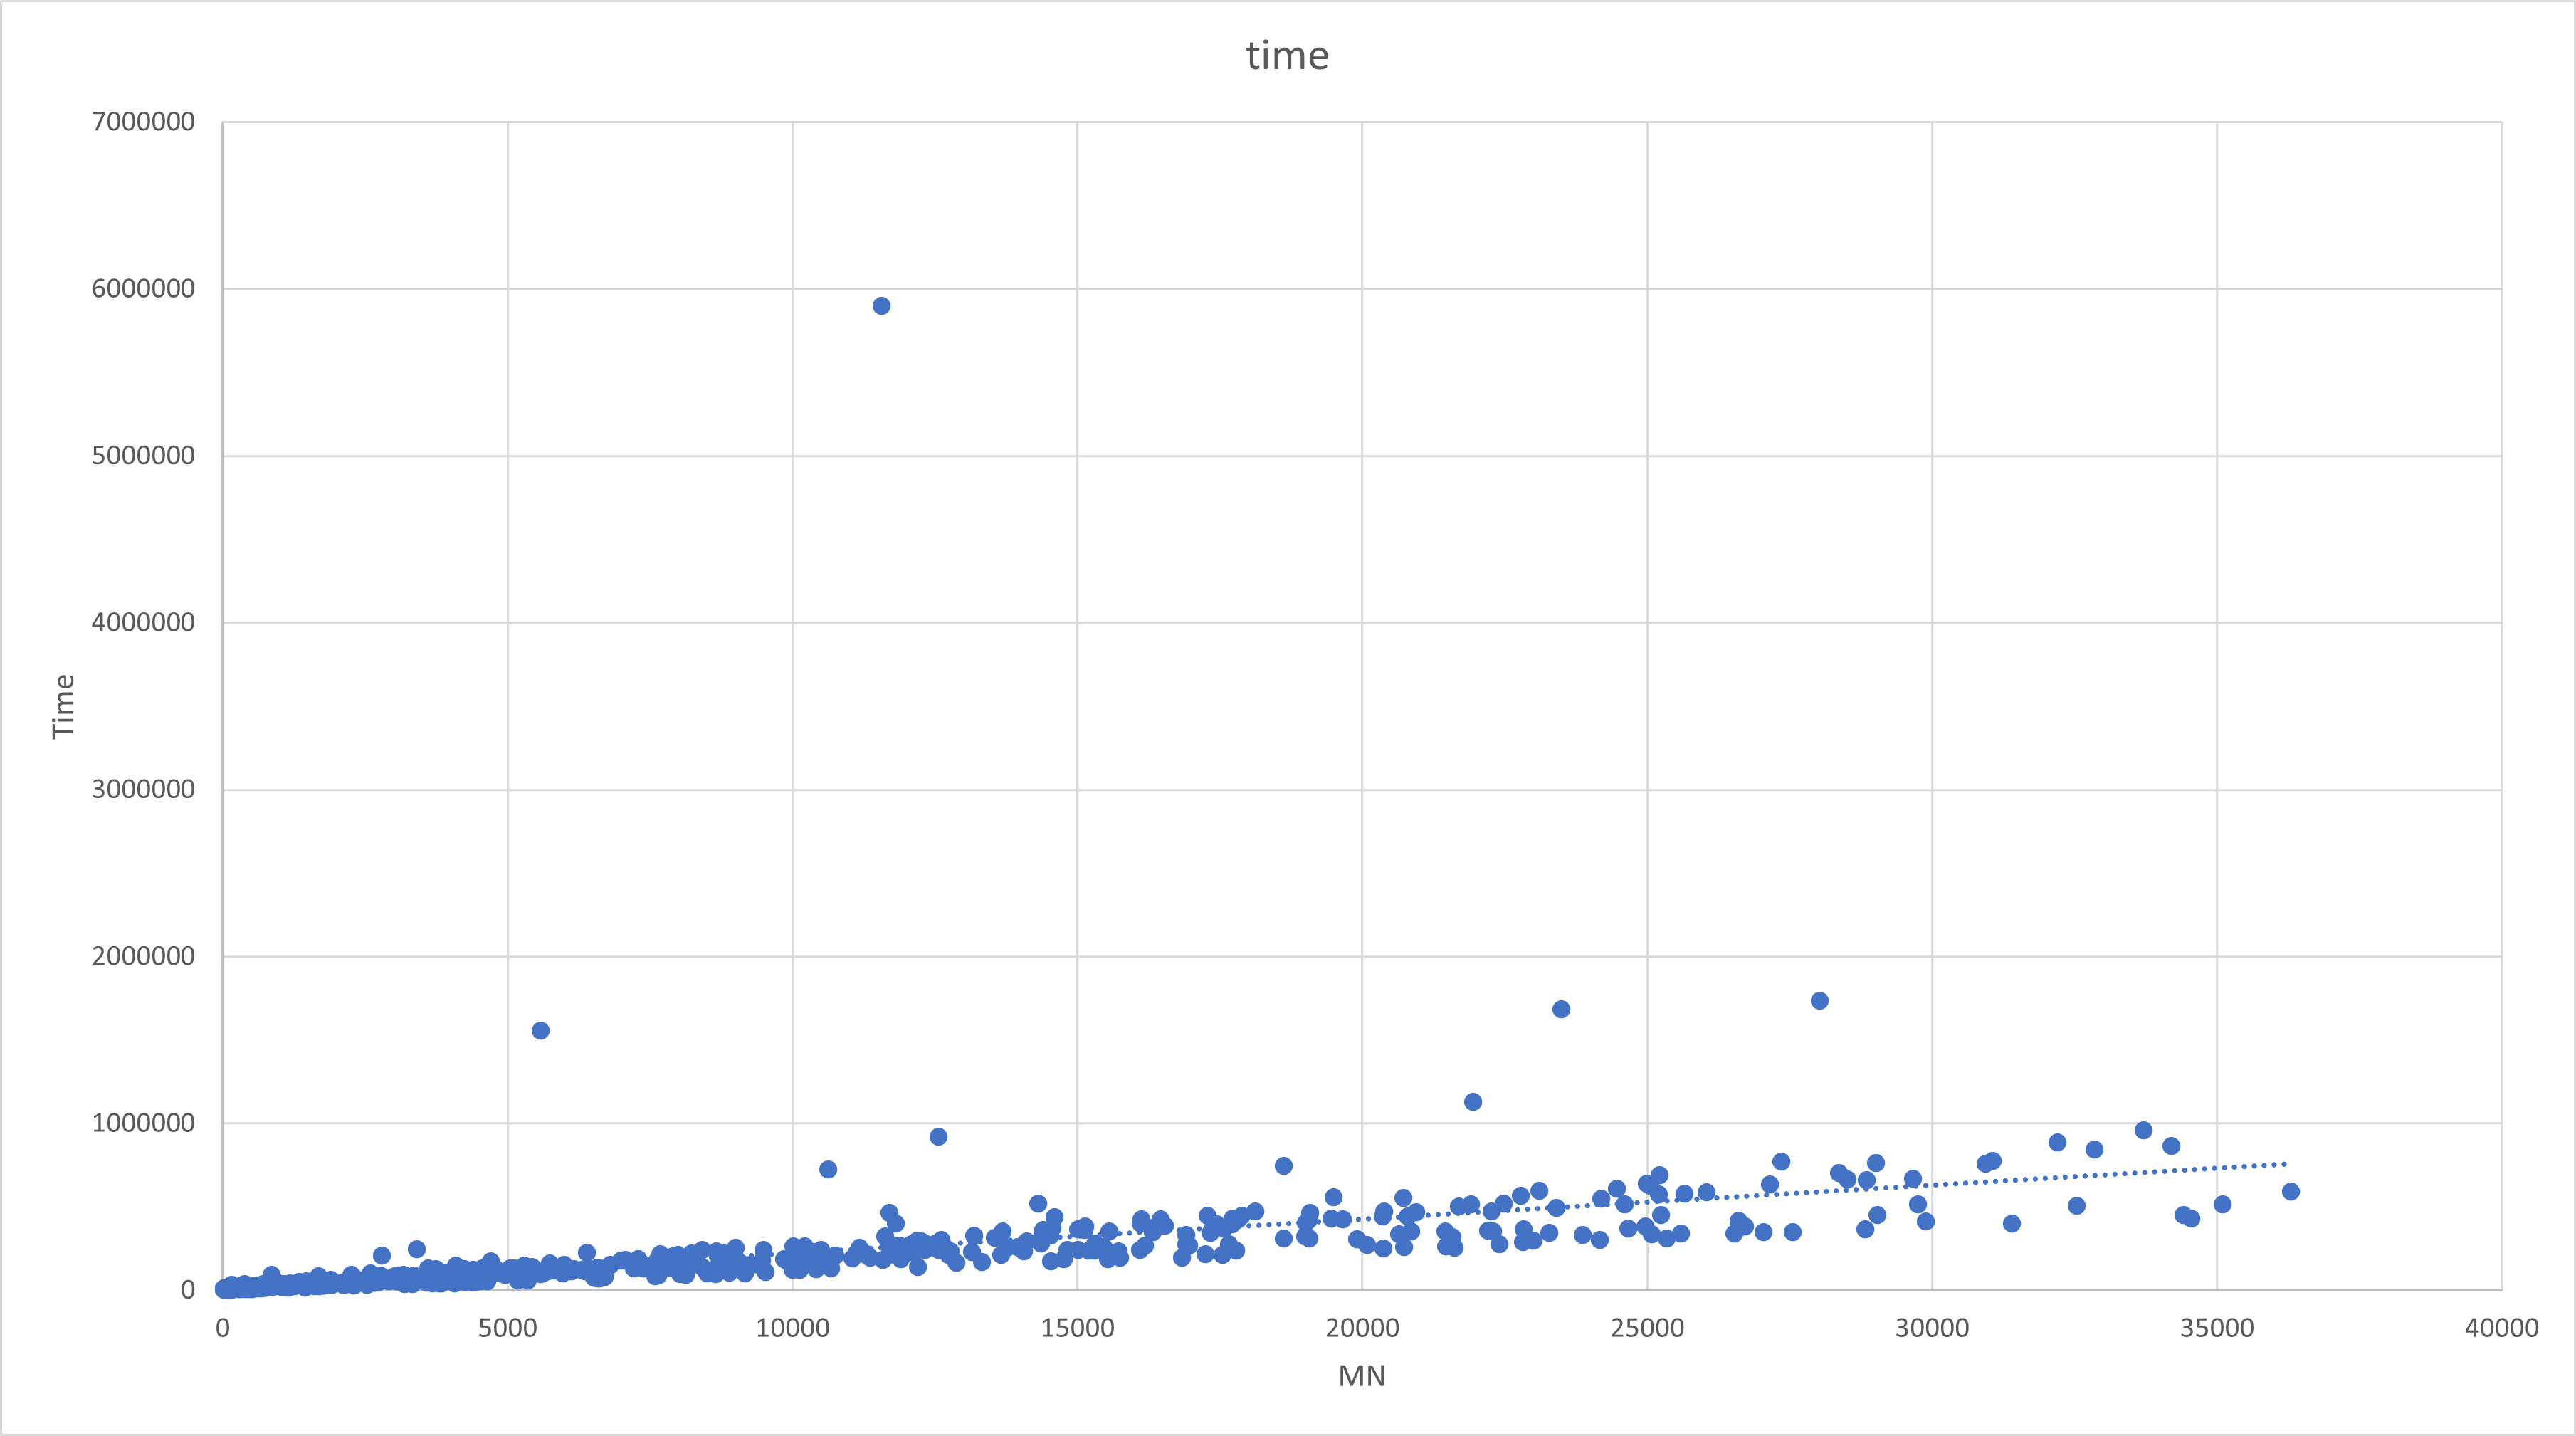
\includegraphics[width=0.7\linewidth]{screen/A1-12}
		\caption{}
		\label{fig:a1-12}
	\end{figure}
	
	
	\noindent First experiment is $w_{i} = 1$ and $\delta = 10$, the last number of the result is the runningtime of milliseconds.  \\
	
	\begin{figure}[H]
		\centering
		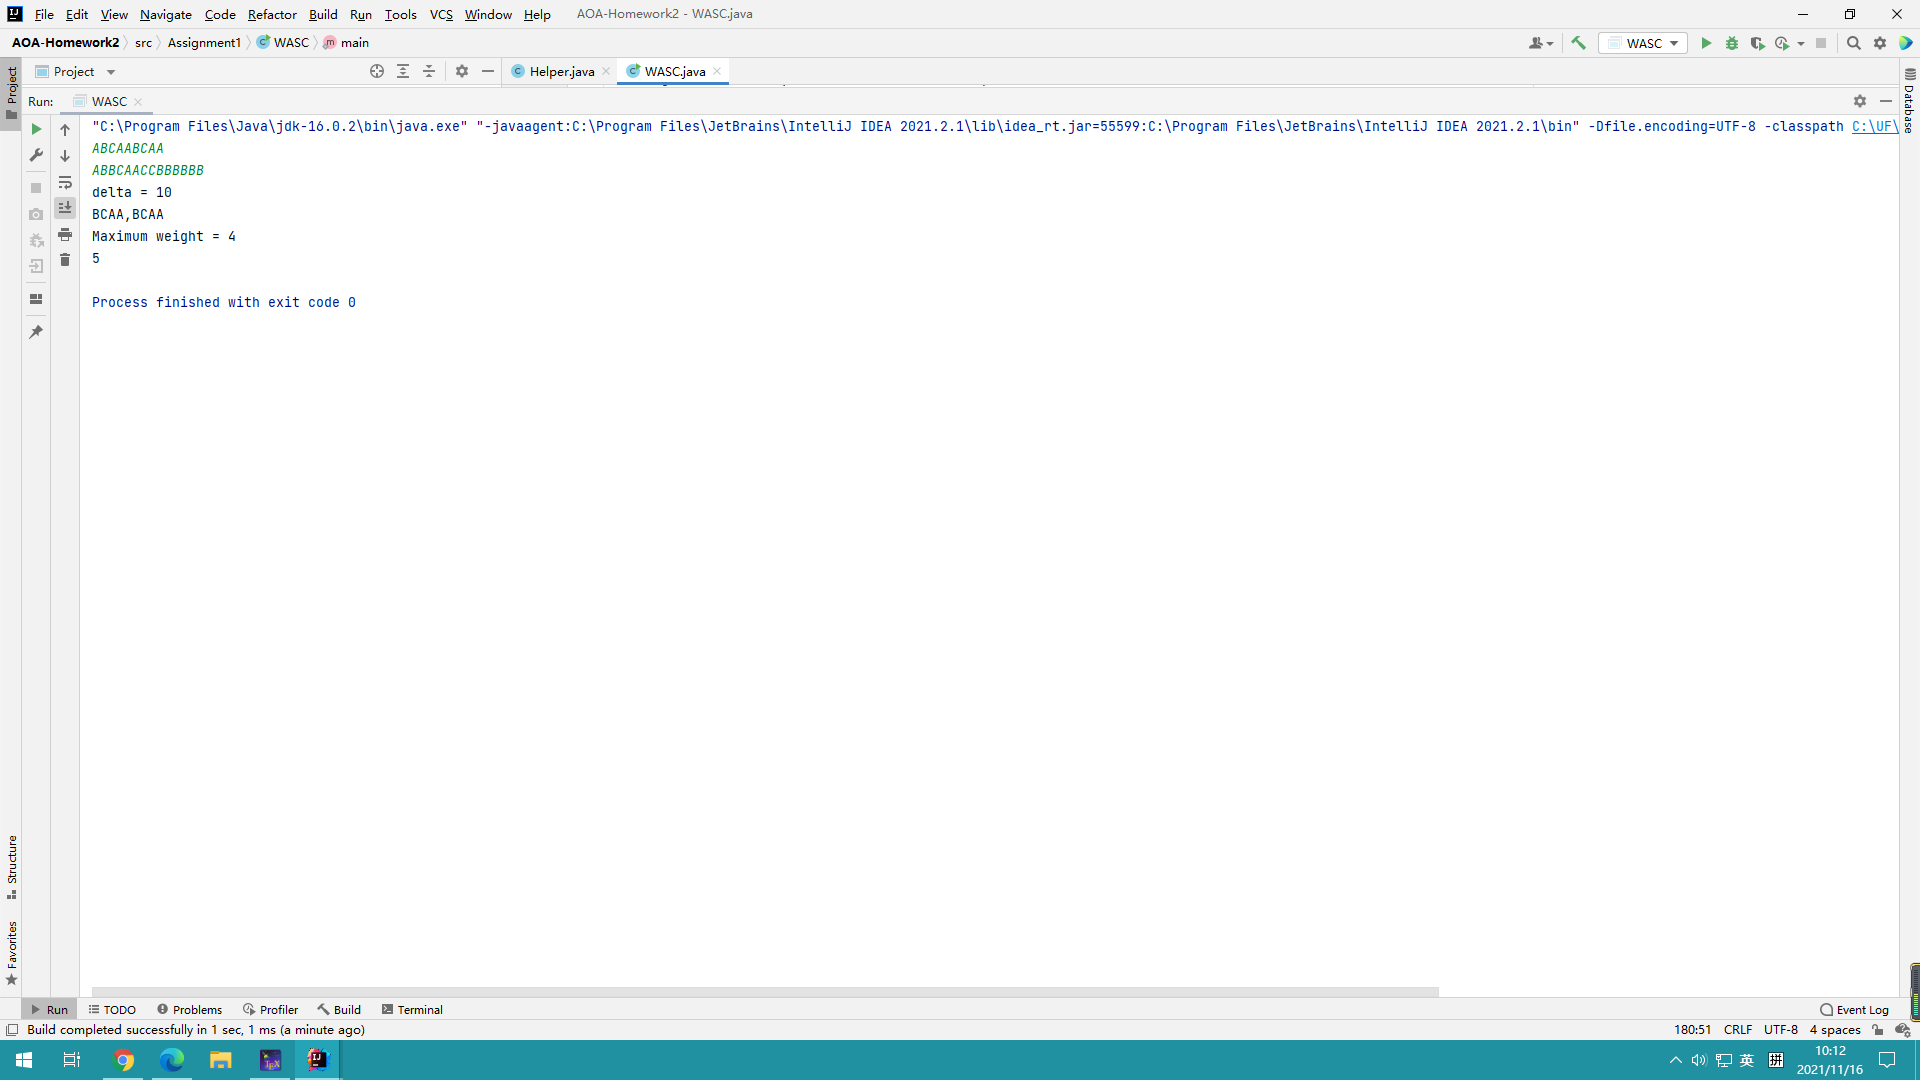
\includegraphics[width=1\linewidth]{screen/A1-1}
		\caption{}
		\label{fig:a1-1}
	\end{figure}
	
	\noindent Here is the ten experiments with different weights and deltas that $w_{i}$ is proportional to the frequency of the letter in English and $\delta$ takes values between the smallest and the largest weight.
	
	\begin{figure}[H]
		\centering
		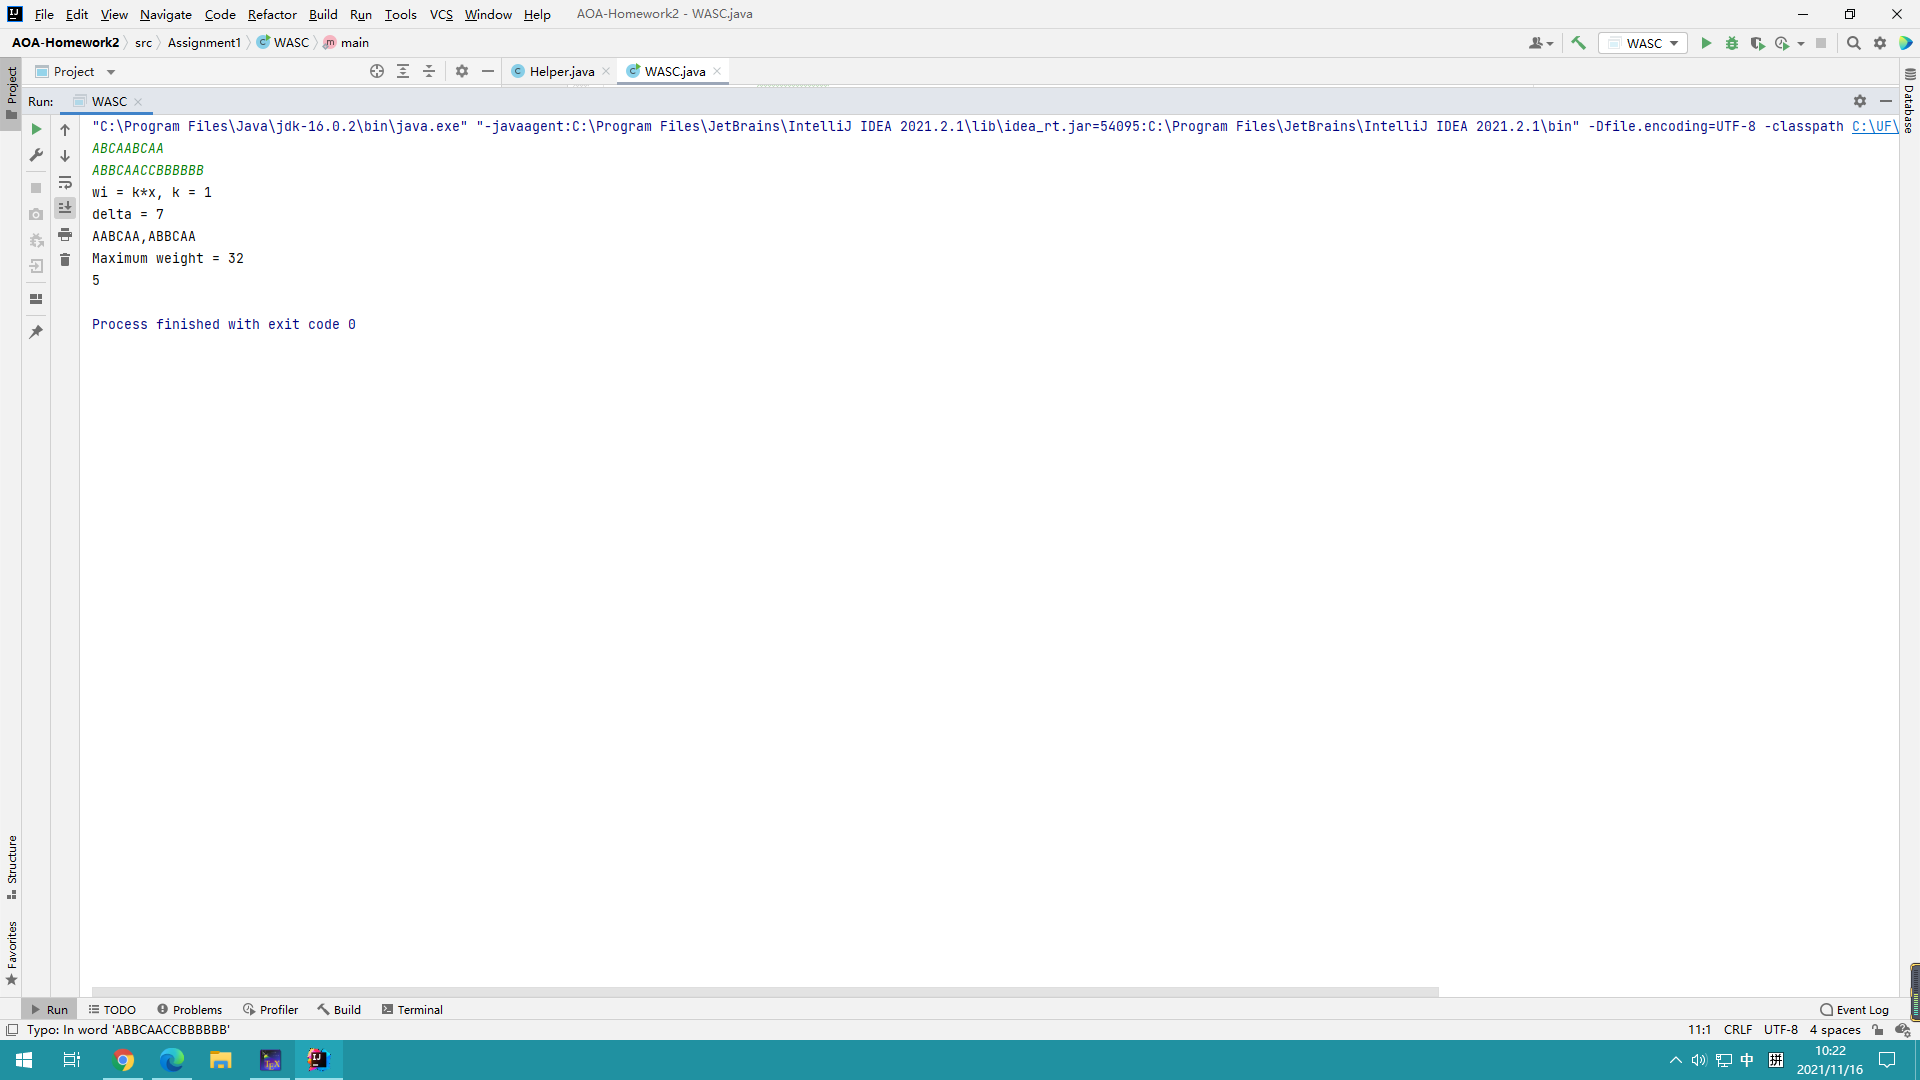
\includegraphics[width=1\linewidth]{screen/A1-2}
		\caption{}
		\label{fig:a1-1}
	\end{figure}

	\begin{figure}[H]
		\centering
		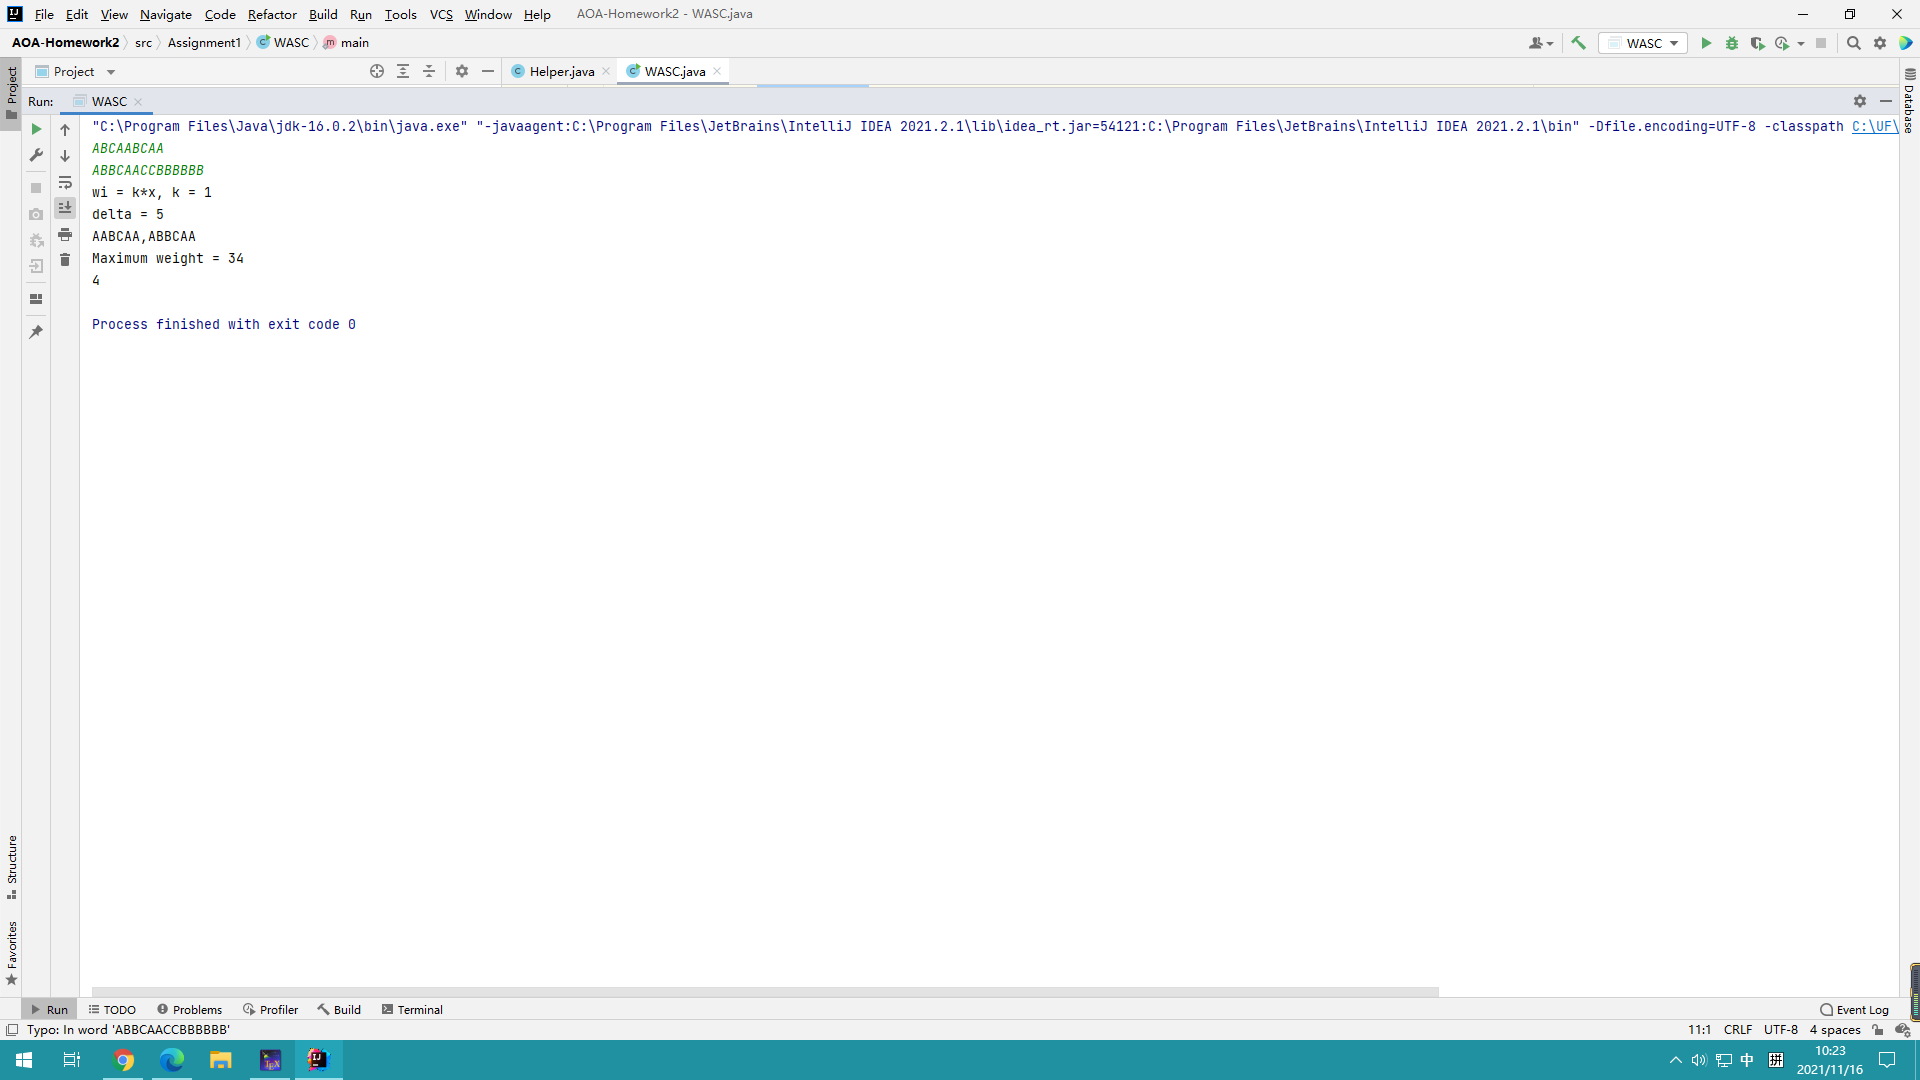
\includegraphics[width=1\linewidth]{screen/A1-3}
		\caption{}
		\label{fig:a1-1}
	\end{figure}
	
	\begin{figure}[H]
		\centering
		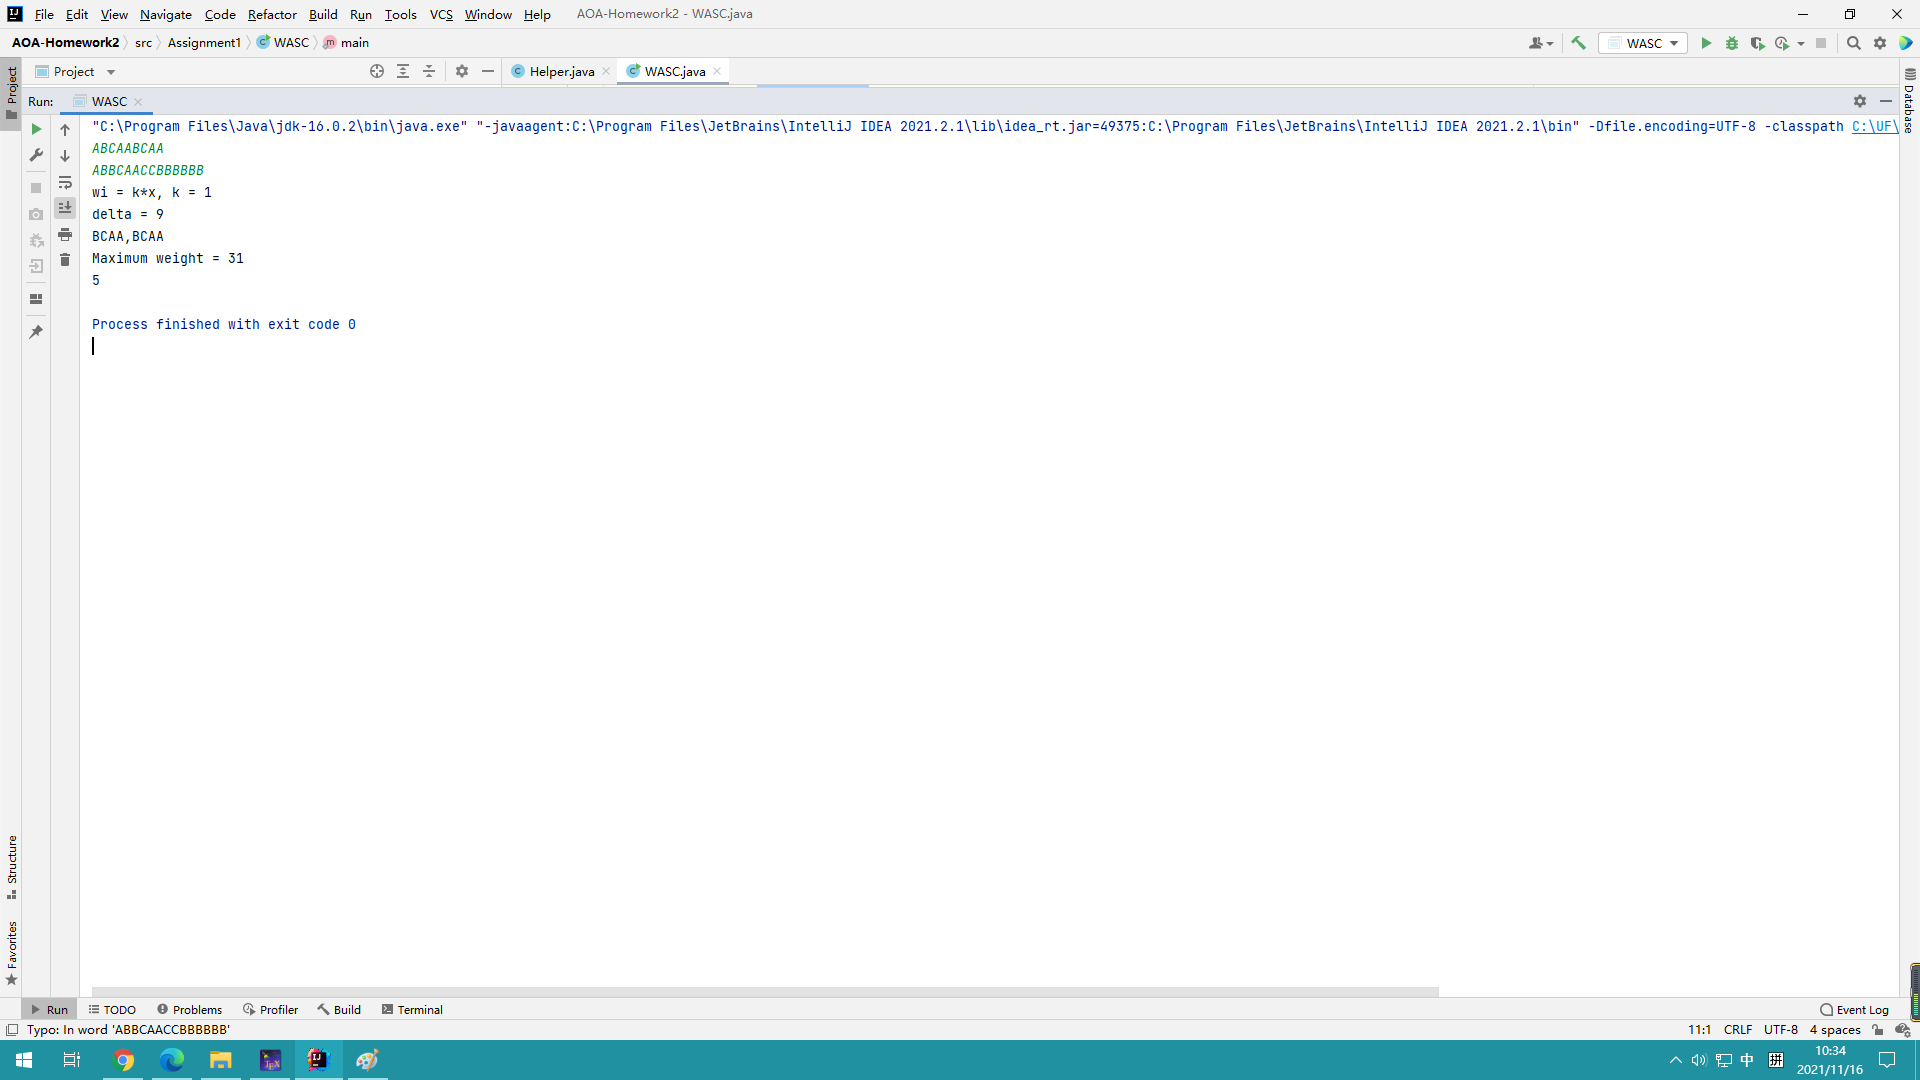
\includegraphics[width=1\linewidth]{screen/A1-11}
		\caption{}
		\label{fig:a1-1}
	\end{figure}
	
	\noindent since the k is 1, there are not so many possible results, so the following results have the k of 2.  \\
	
	\begin{figure}[H]
		\centering
		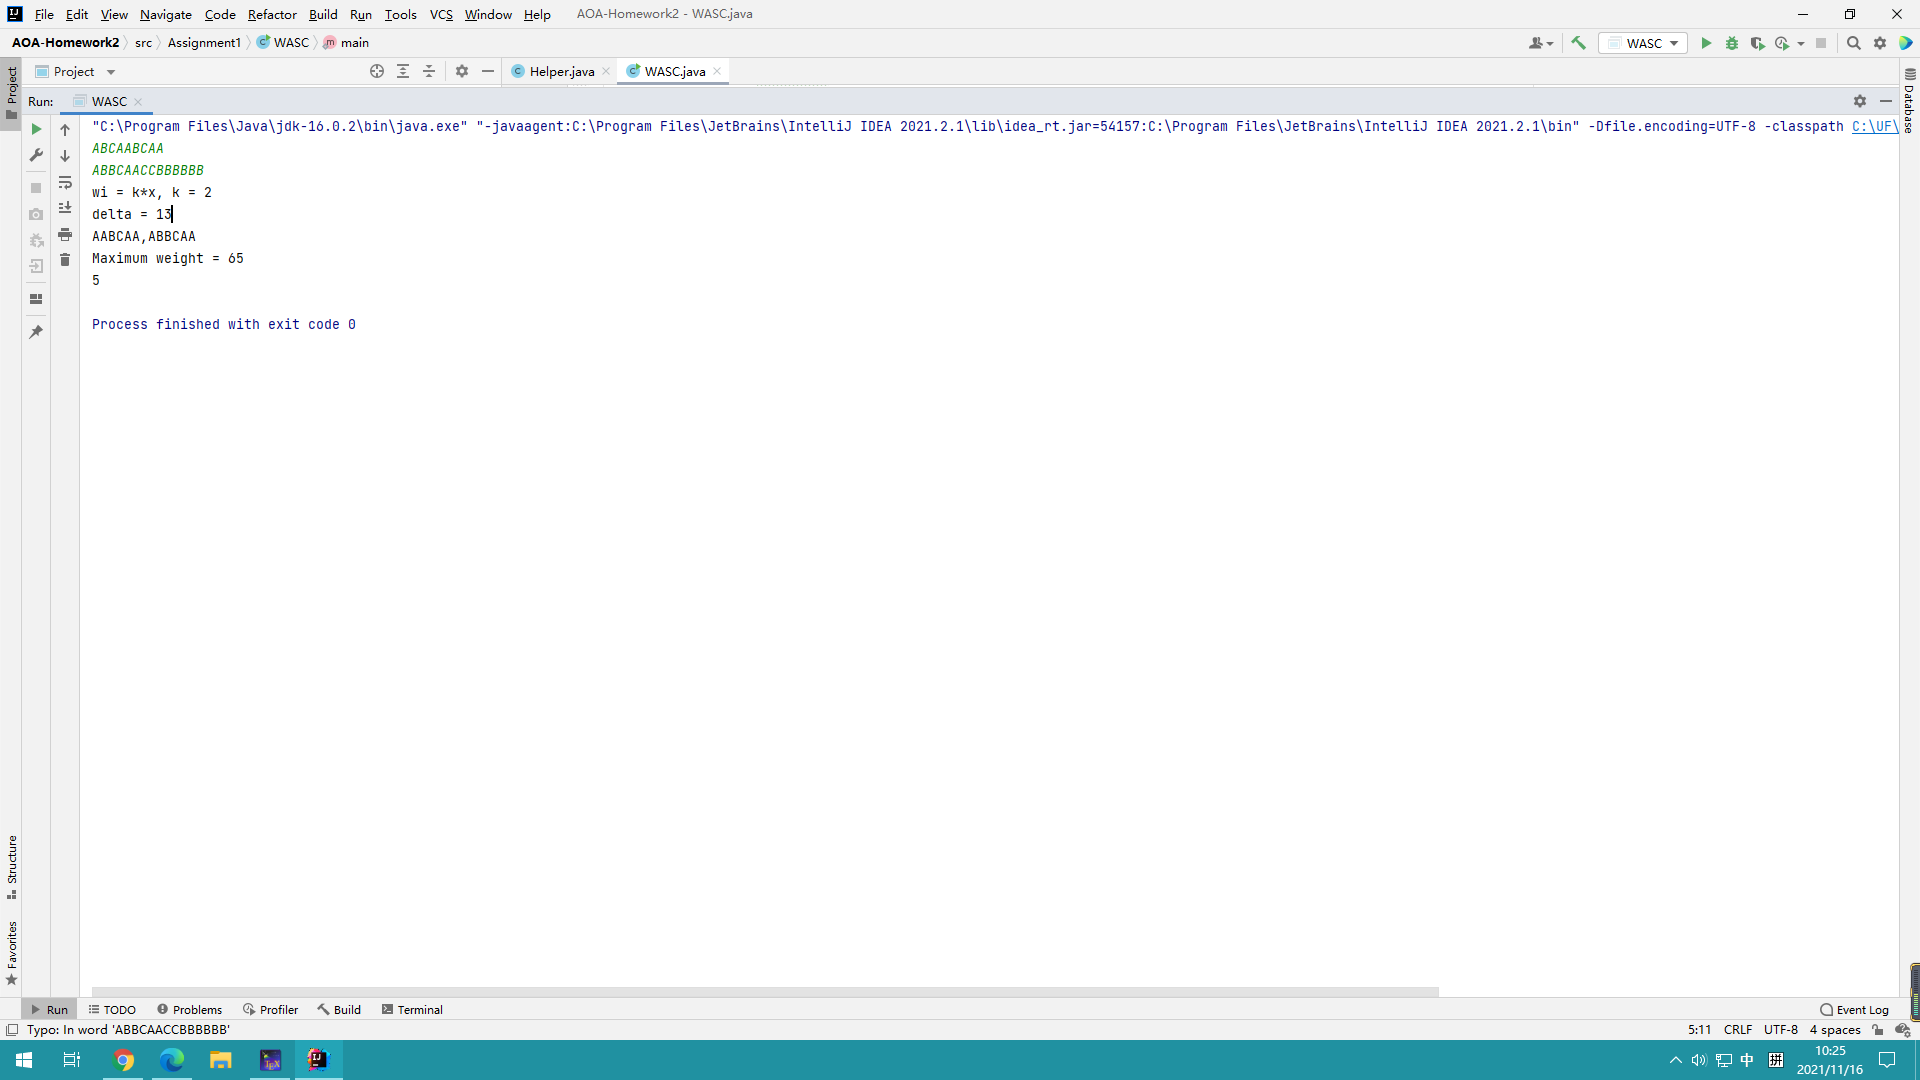
\includegraphics[width=1\linewidth]{screen/A1-4}
		\caption{}
		\label{fig:a1-1}
	\end{figure}
	
	\begin{figure}[H]
		\centering
		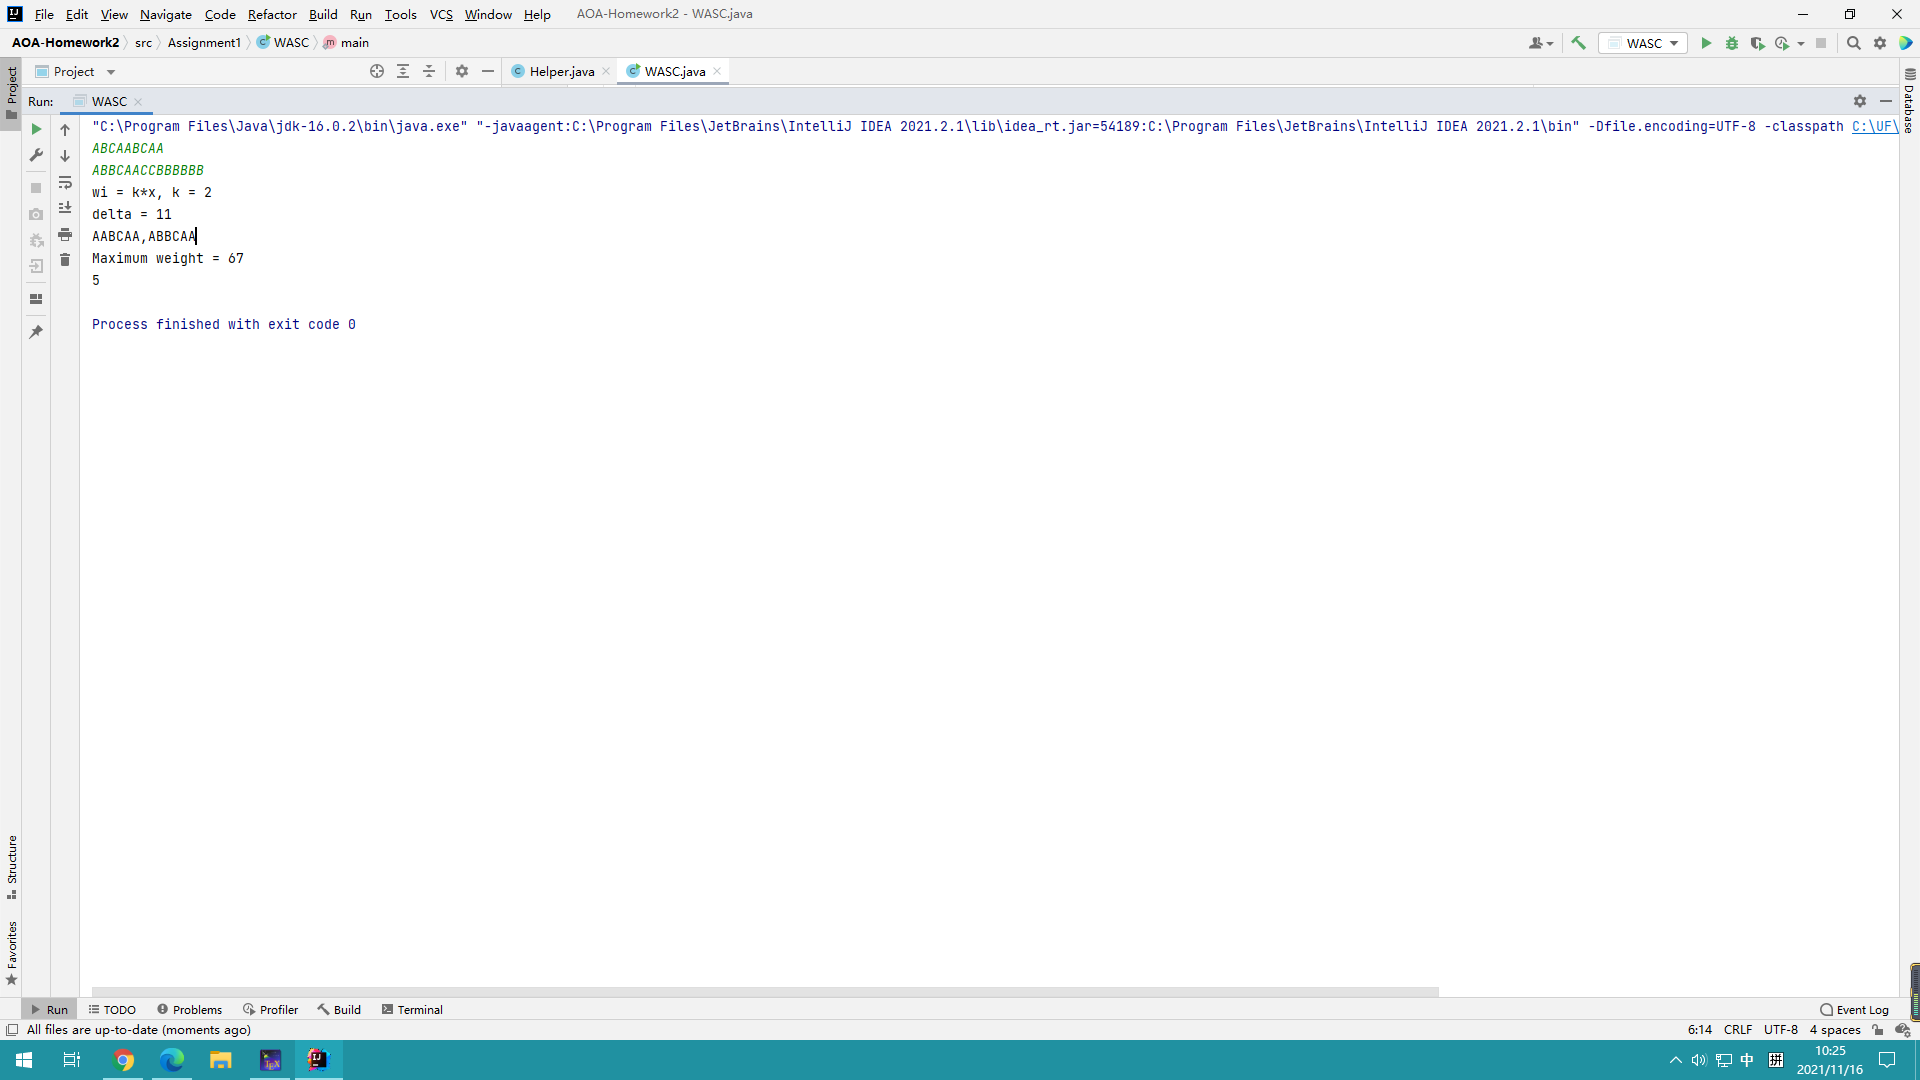
\includegraphics[width=1\linewidth]{screen/A1-5}
		\caption{}
		\label{fig:a1-1}
	\end{figure}
	
	\begin{figure}[H]
		\centering
		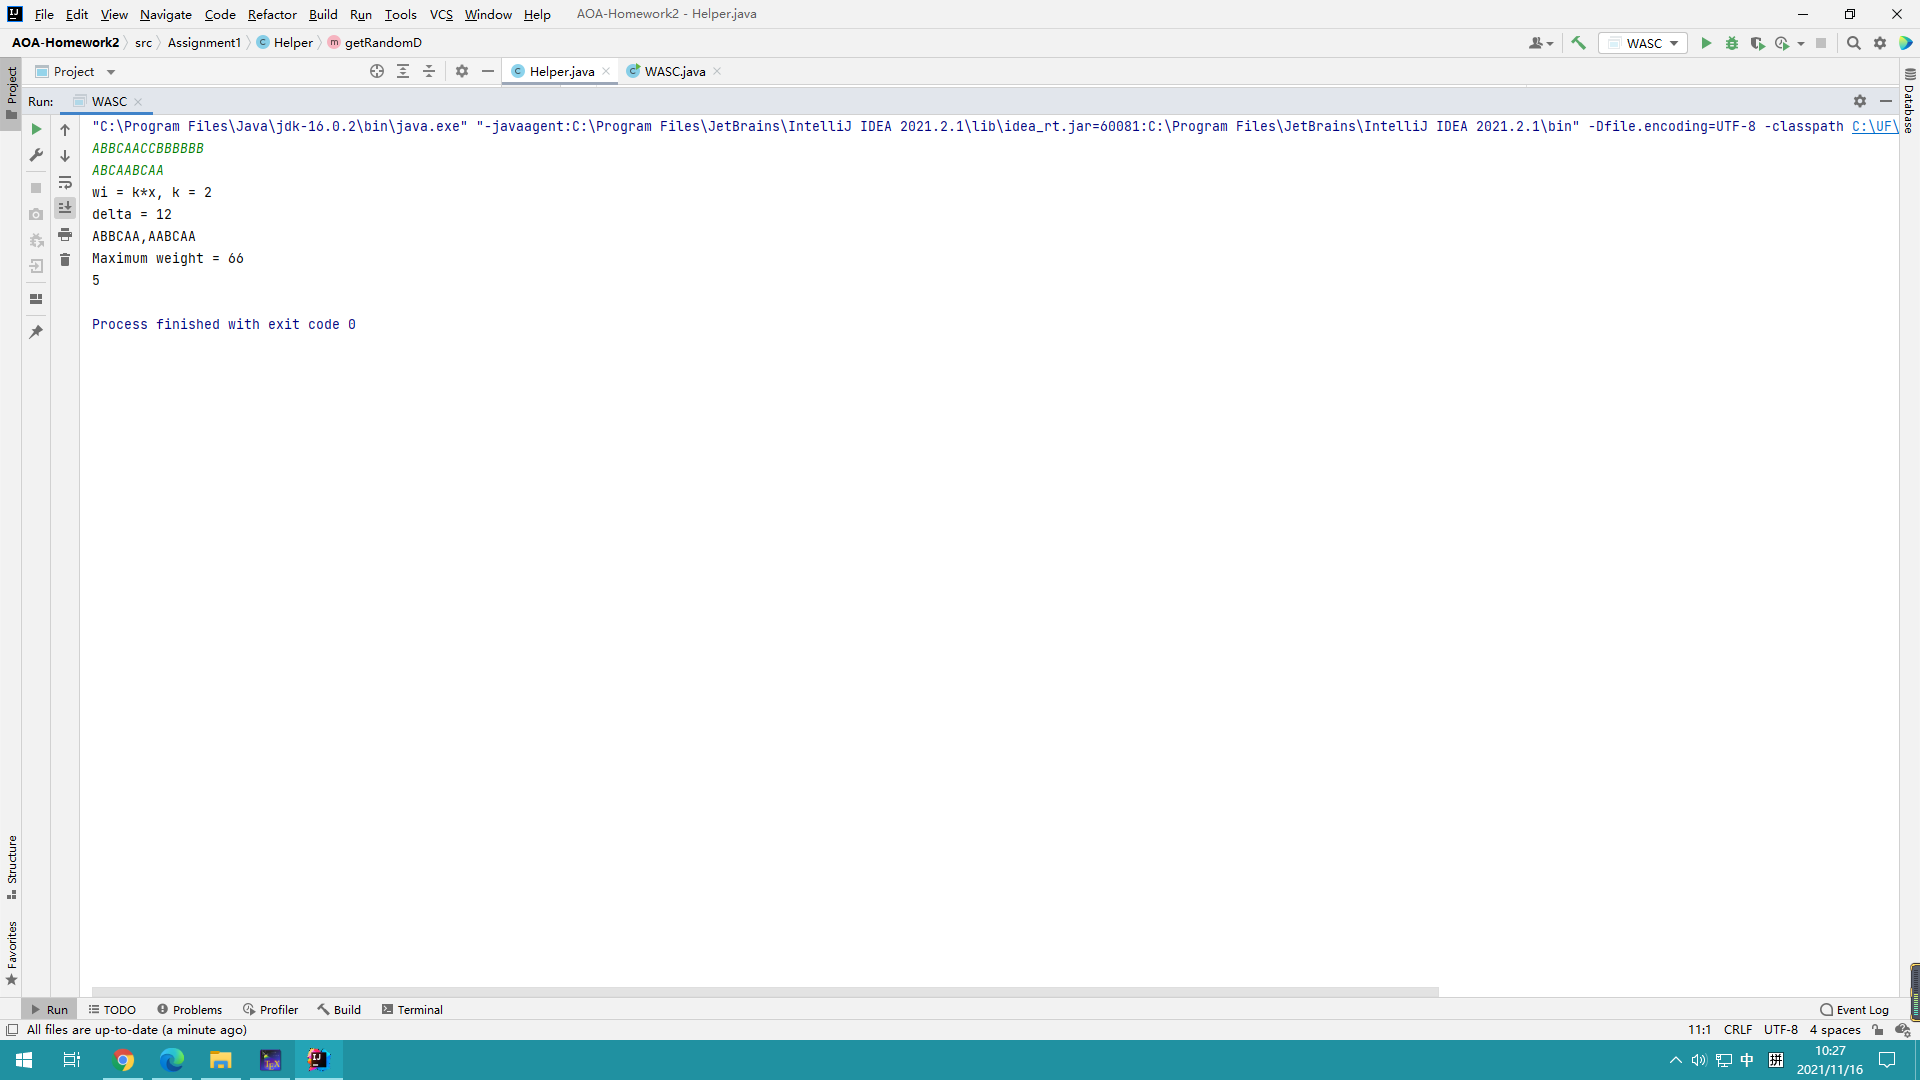
\includegraphics[width=1\linewidth]{screen/A1-6}
		\caption{}
		\label{fig:a1-1}
	\end{figure}
	
	\begin{figure}[H]
		\centering
		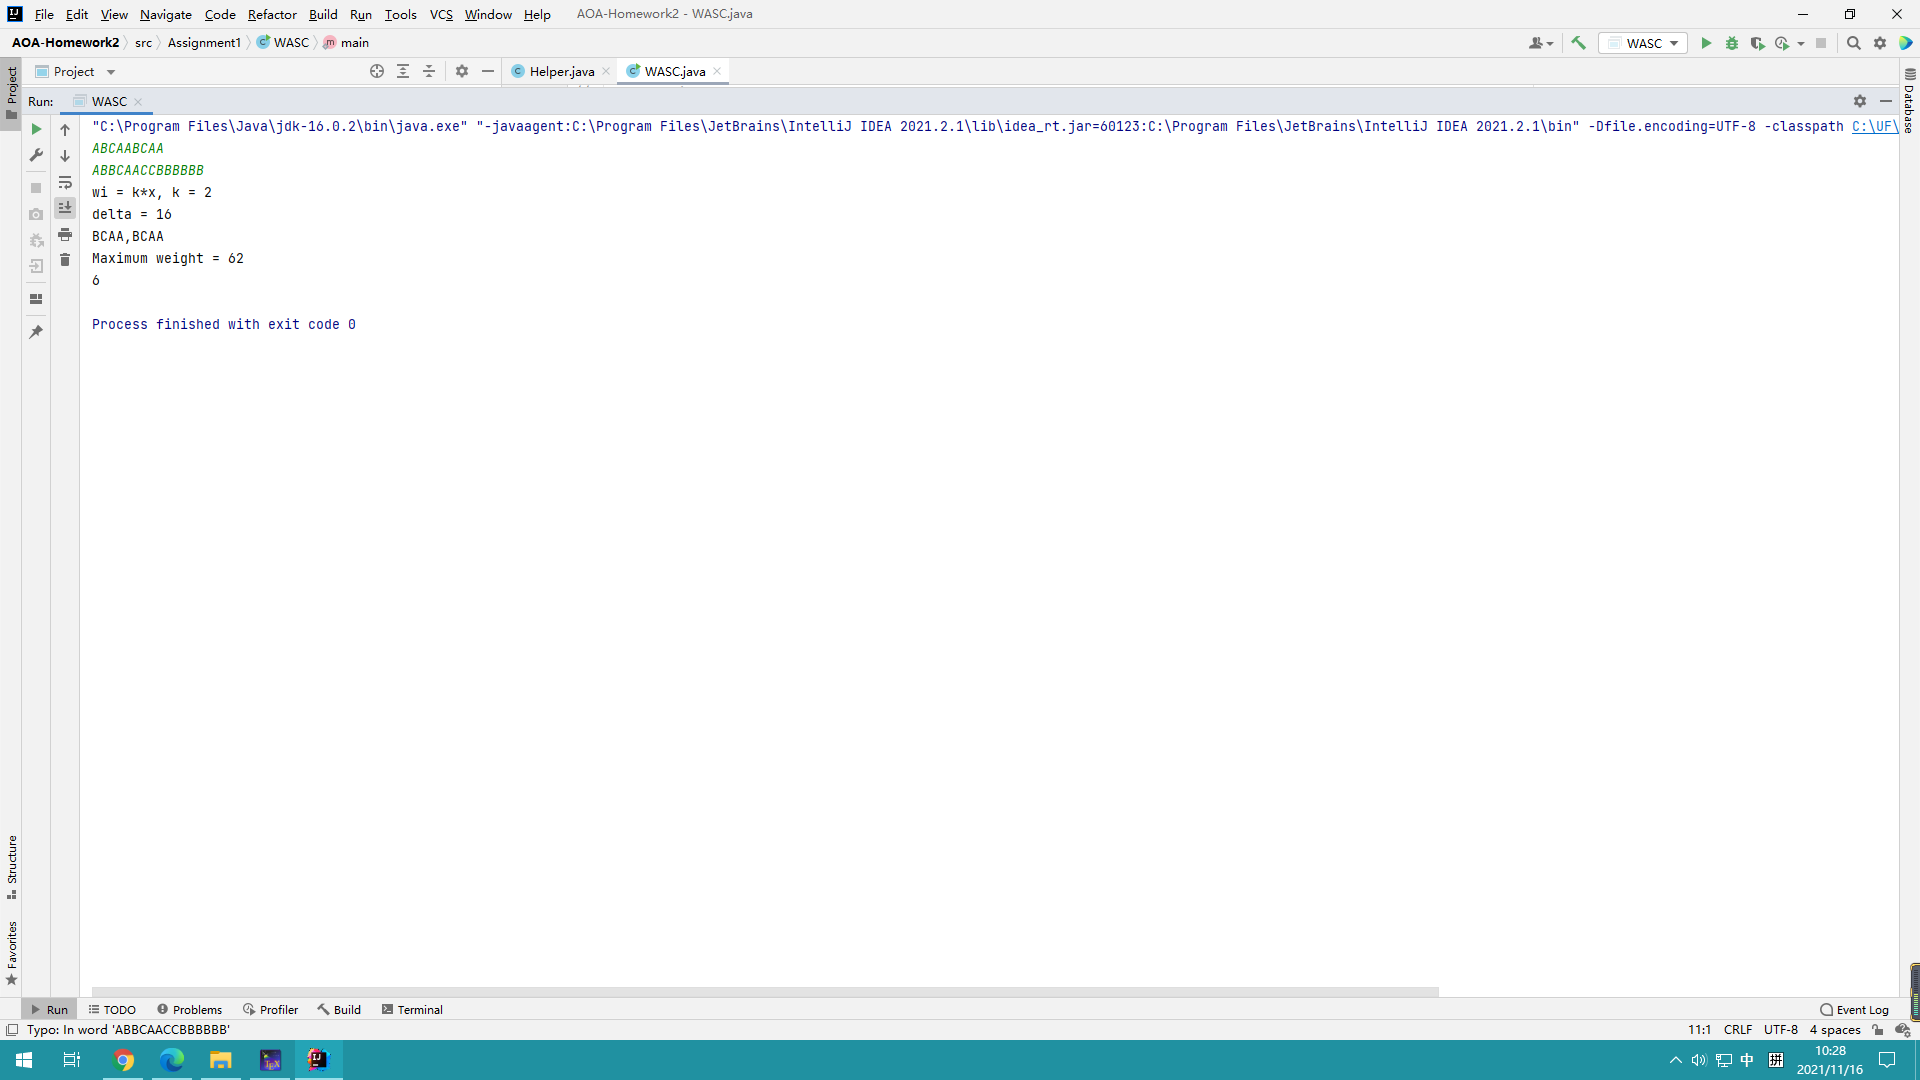
\includegraphics[width=1\linewidth]{screen/A1-7}
		\caption{}
		\label{fig:a1-1}
	\end{figure}
	
	\begin{figure}[H]
		\centering
		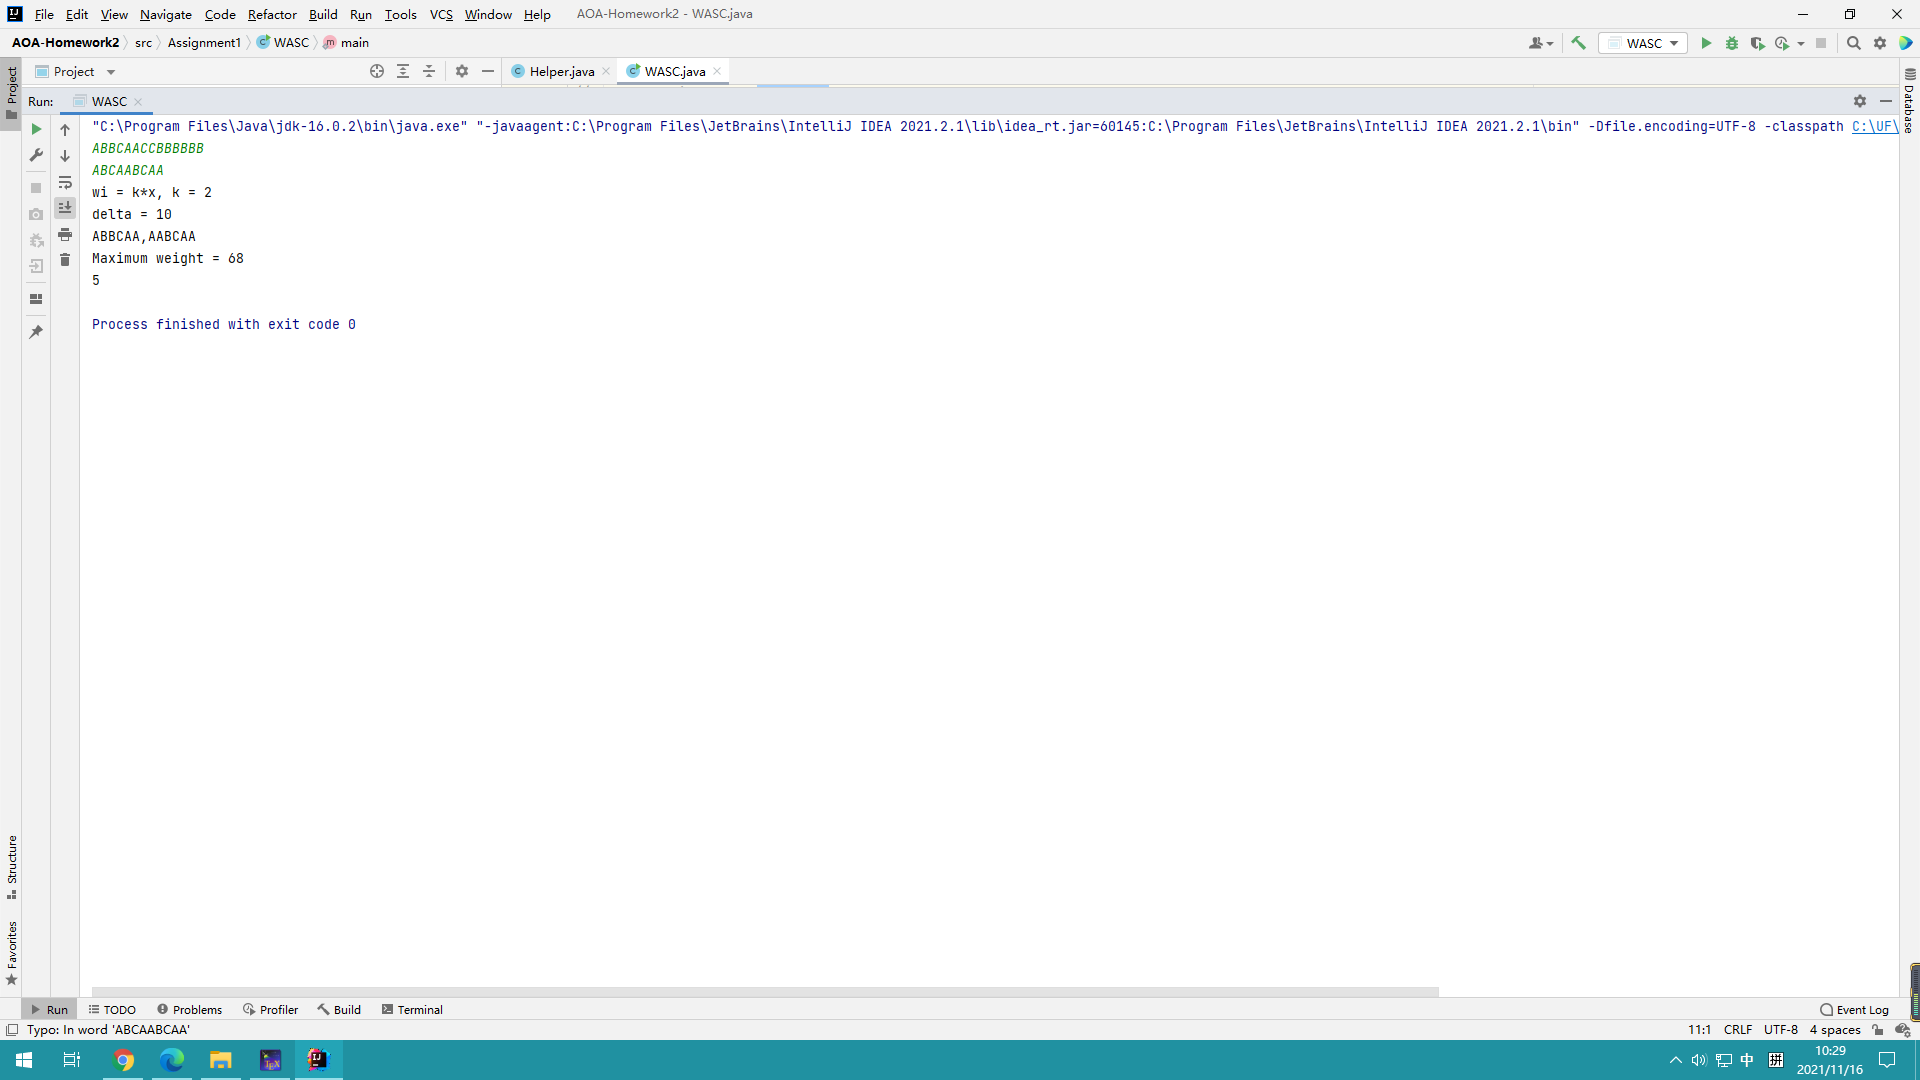
\includegraphics[width=1\linewidth]{screen/A1-8}
		\caption{}
		\label{fig:a1-1}
	\end{figure}
	
	\begin{figure}[H]
		\centering
		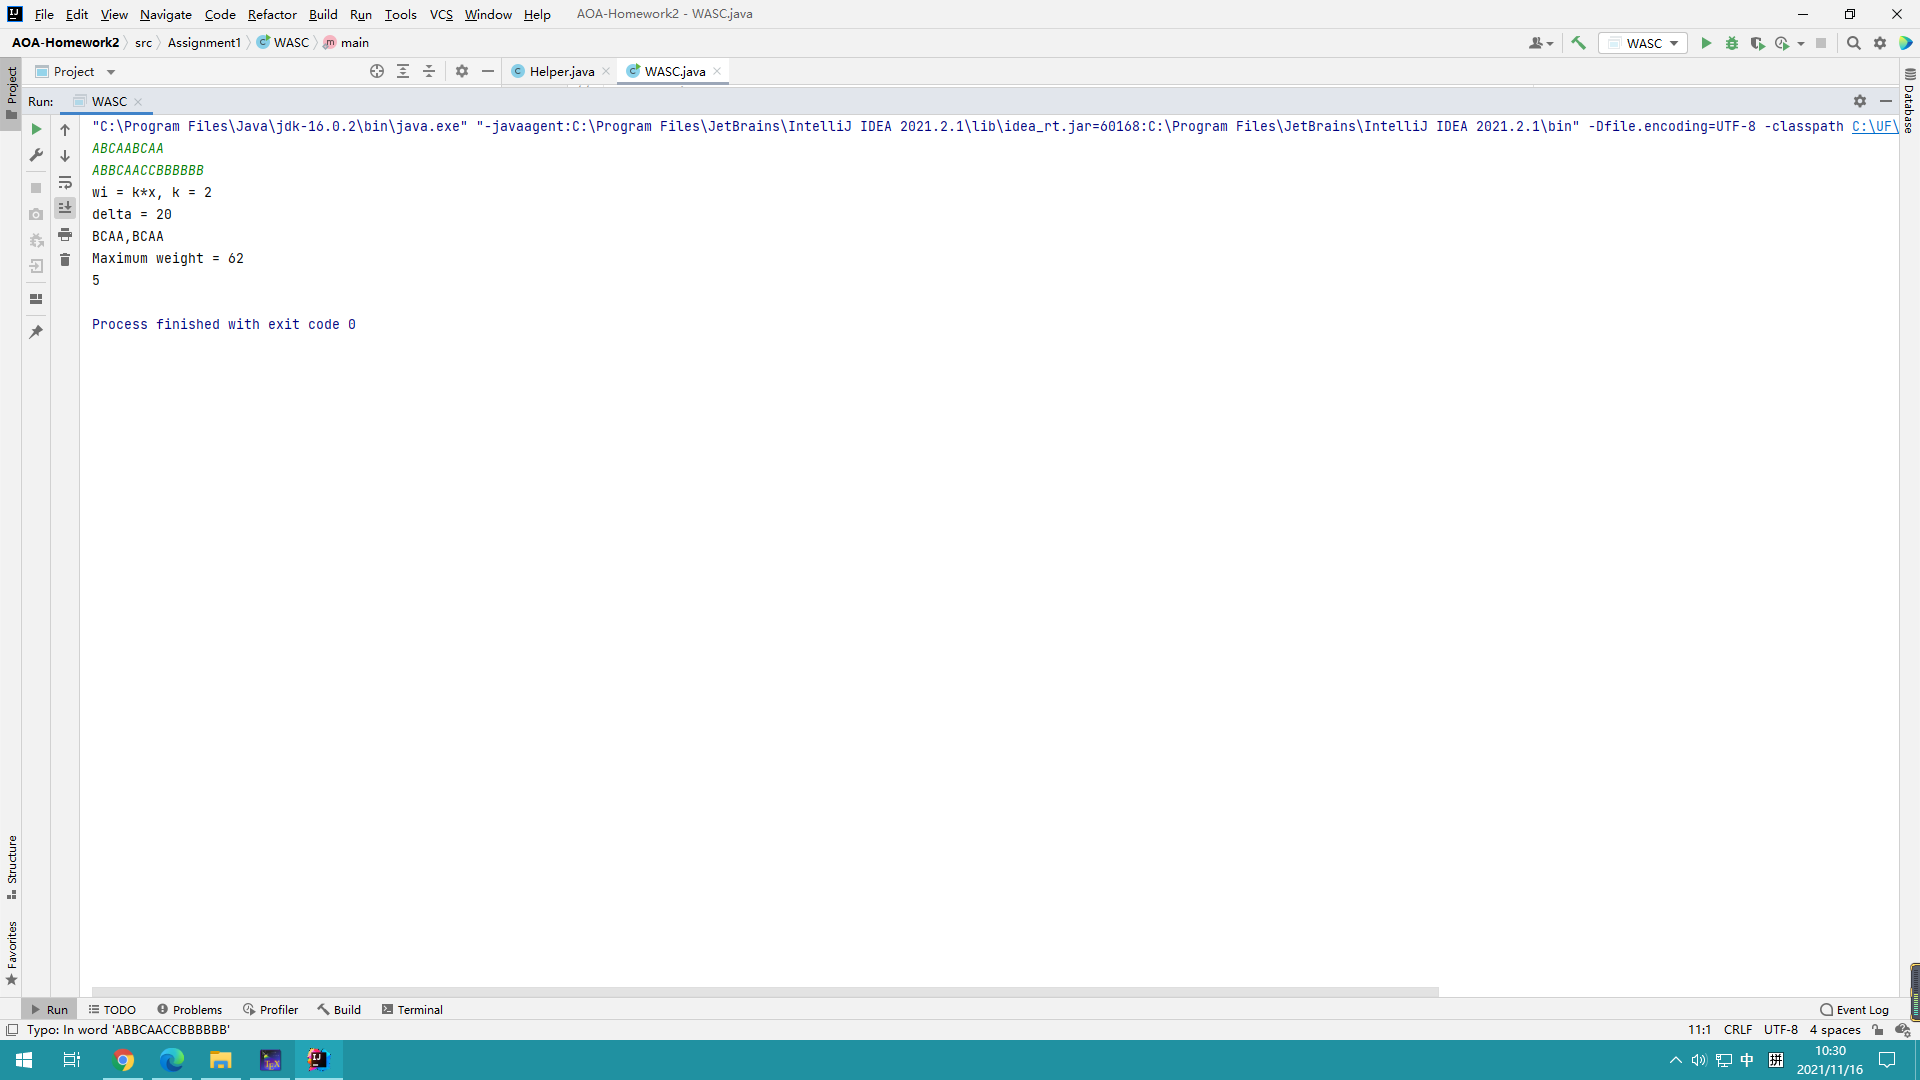
\includegraphics[width=1\linewidth]{screen/A1-9}
		\caption{}
		\label{fig:a1-1}
	\end{figure}
	
	\begin{figure}[H]
		\centering
		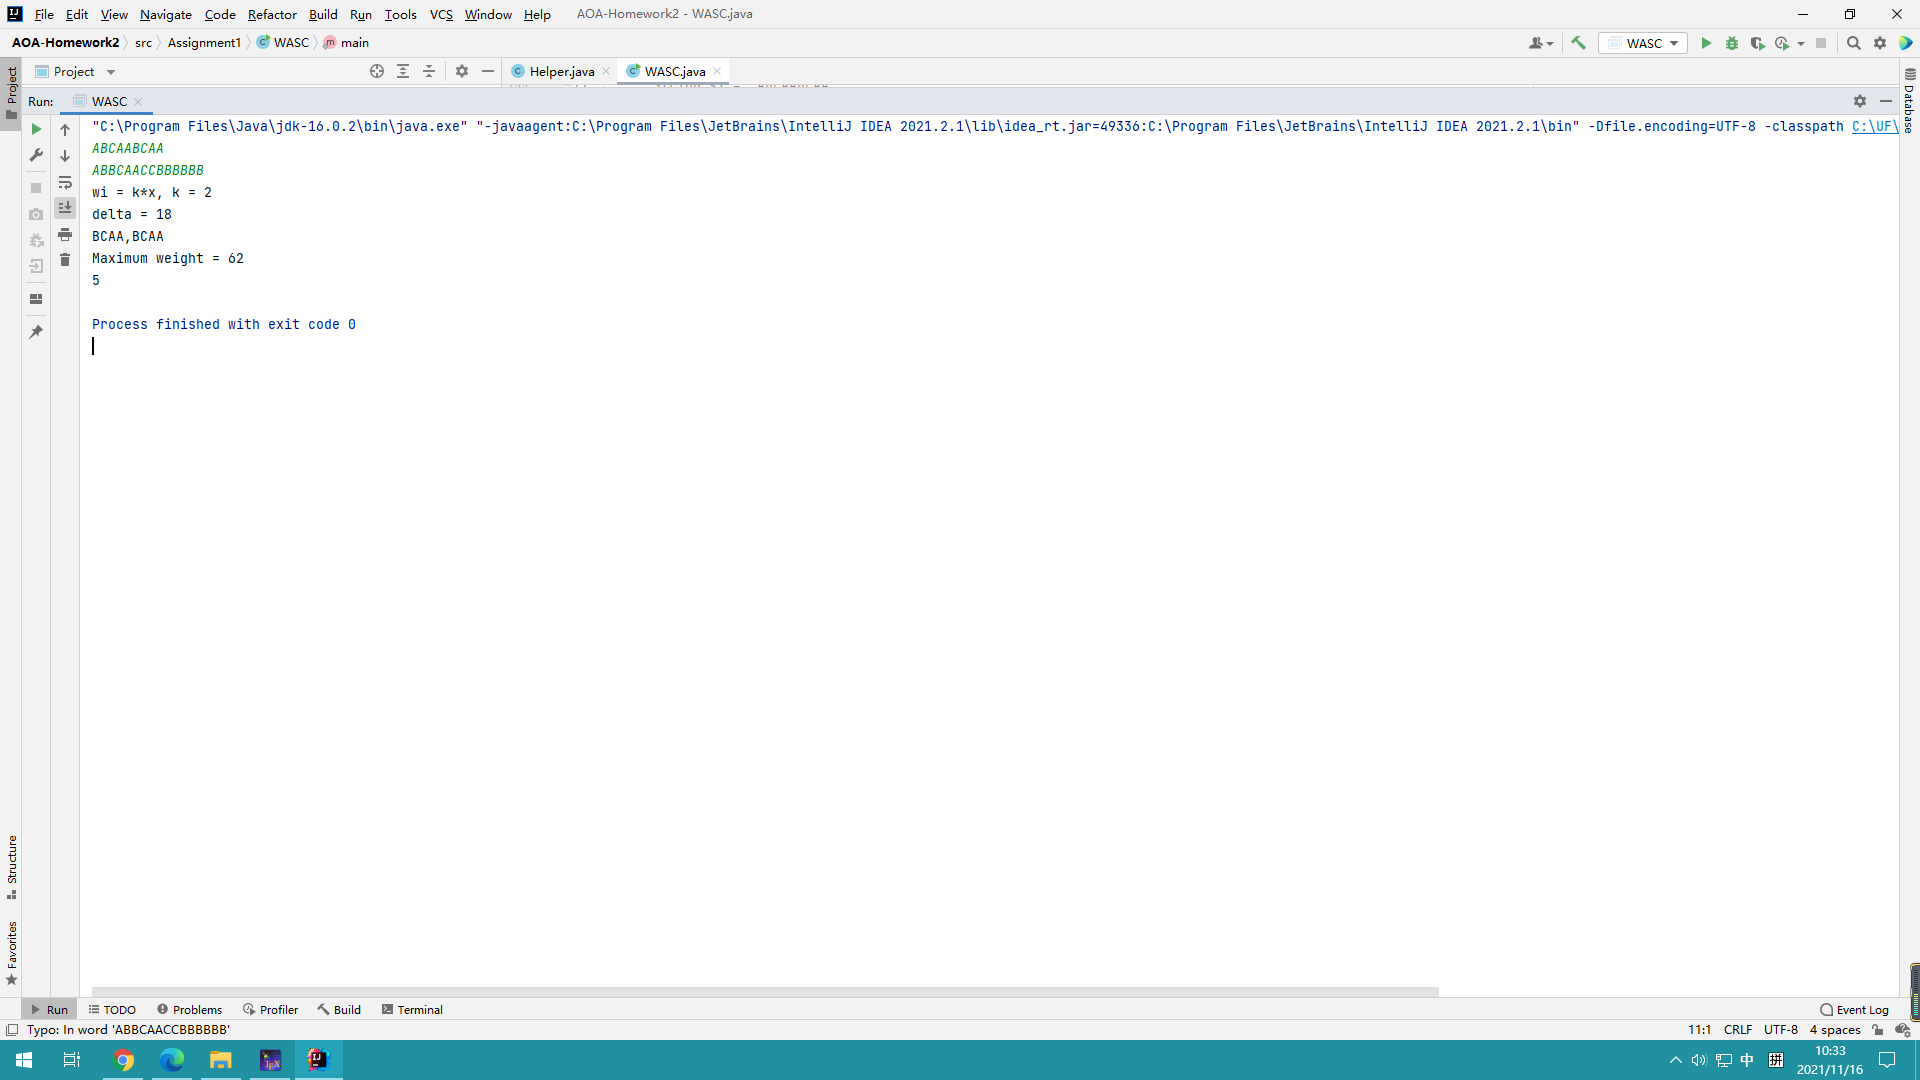
\includegraphics[width=1\linewidth]{screen/A1-10}
		\caption{}
		\label{fig:a1-1}
	\end{figure}

	 
	
	\clearpage
	
	\section{Problem 2: Interval-based constant best approximation}
	\subsection{Pseudo-code of the Algorithm}
	\begin{algorithm}  
		\caption{best approximation}  
		\begin{algorithmic} 
			\Require a set of points \{$p_{1}$,...,$p_{n}$\}  
			\Ensure
			\State Initially let M[n] be the array to memorize the minimum cost M[i] for each i, 0$\leq$i$\leq$n.
			\State let M[0] = 0
			\For{j = 1 to n}
				\For{i = 1 to j}
					\State compute the least error $e_{ij}$ for each interval from point $p_{i}$ to $p_{j}$
				\EndFor
			\EndFor
			
			\For{j = 1 to n}
				\State M[j] = $min_{1\leq i\leq j}$($e_{ij}$ + $\delta$ + M[i-1])
			\EndFor
		\end{algorithmic}  
	\end{algorithm} 
	
	\subsection{Proof of the algorithm's correctness}
	
	Since the goal is to find a partitioning of the interval [1,M] into contiguous intervals such that the error of approximating points in each interval element by the average value of y in the interval is minimized. \\ 
	
	\noindent Firstly, we can get the equation from the class recording that the minimum error of these points is: \\ 
	
	$E^{2} = \sum_{i=1}^n (y_{i})^2 - \frac{(\sum_{i=1}^n y_{i})^2}{n}$    \\   
	
	\noindent Then, we assume that for the index j, [i,j] is the last interval that we divided, so we can get the bellman equation that relate OPT(j) and OPT(i-1). \\  
	
	\noindent Bellman equation: \\
	
	OPT(j) =
	$\begin{cases} 
		0,  & \mbox{if }\mbox{j = 0} \\
		min_{1\leq i\leq j} \{e(i,j) + \delta + OPT(i-1)\}, & \mbox{otherwise}
	\end{cases}$ \\
	
	
	\subsection{Algorithm's running time}
	According to the pseudo-code, if we want to compute the complexity of the Algorithm, we need to consider two parts.\\
	
	\noindent The first part is computing the least error $e_{ij}$ for each $p_{i}$ to $p_{j}$. According to the equation, for each pair of i and j, we need O(n) to compute the sum of $y_{i}^{2}$ and the sum of y, and it only takes O(1) to put them together and get $E^{2}$. So to get all $e_{ij}$, it needs $O(n^{3})$. \\
	
	\noindent The second part is the get the M[i] for each i from 1 to n. For each i, we need to compute the minimum cost of the sum of $e(i,j) + \delta + OPT(i-1)$, and it takes O(n) times. So the second part takes $O(n^{2})$.  \\
	
	\noindent To conclude, the total complexity of the algorithm takes $O(n^{3})$.  \\
	
	\noindent Here is the memory condition of the program that is solved by using array. \\
	
	\begin{figure}[H]
		\centering
		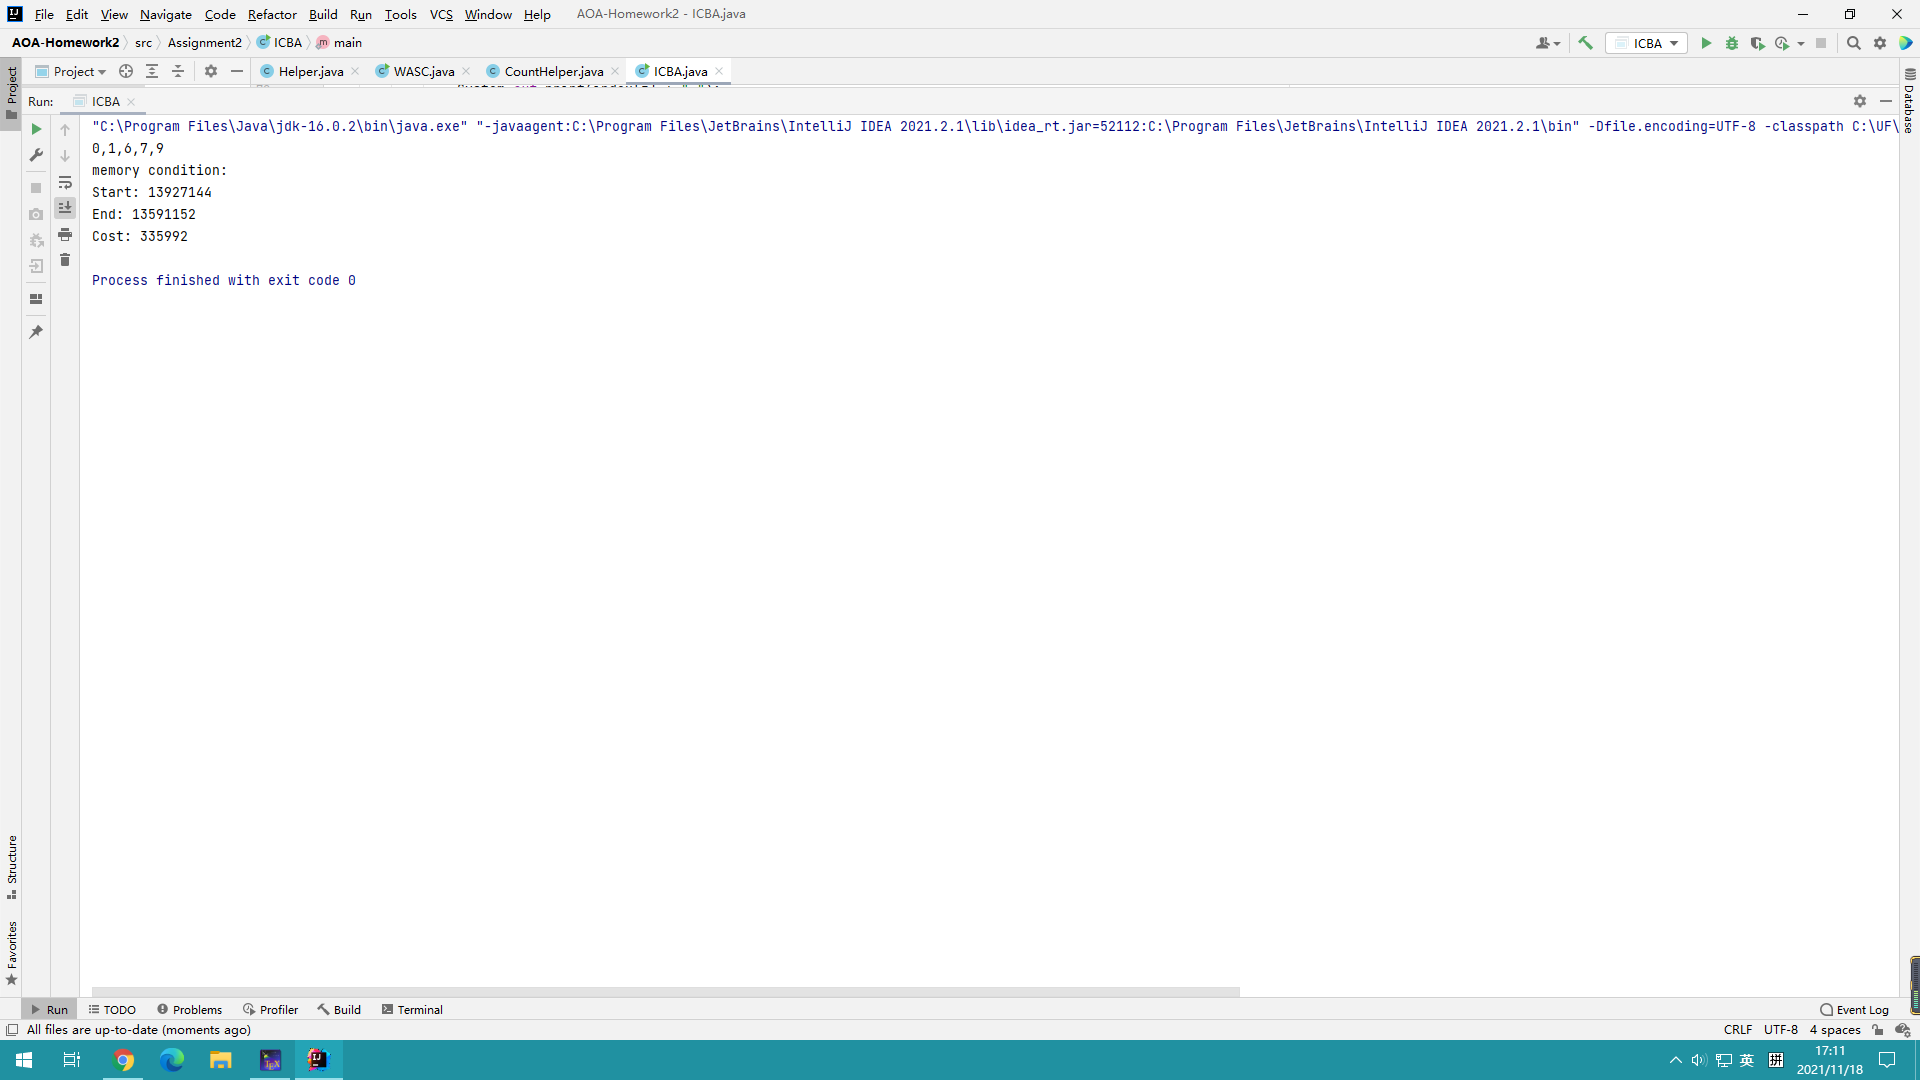
\includegraphics[width=1\linewidth]{screen/A2-1}
		\caption{}
		\label{fig:a2-1}
	\end{figure}
	
	\noindent Here is the memory condition of the program that is solved by using hashmap. \\
	
	\begin{figure}[H]
		\centering
		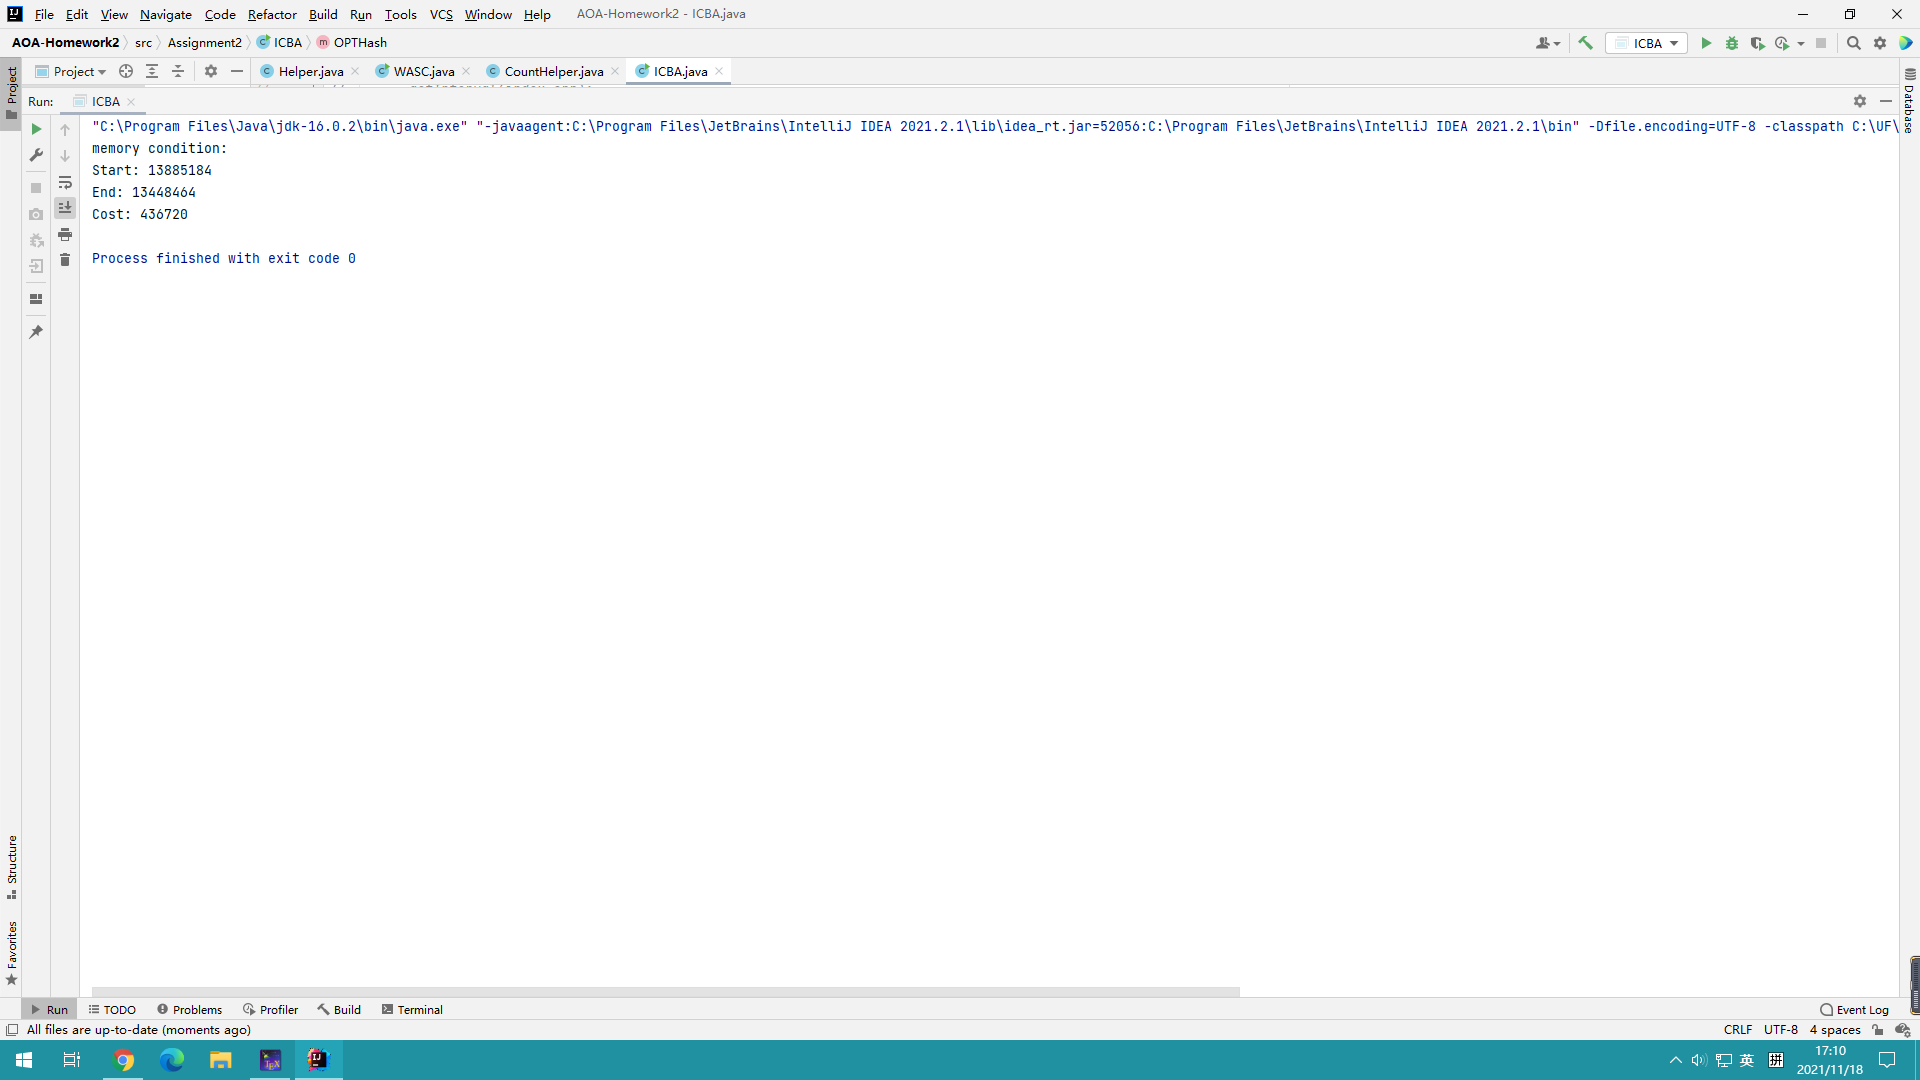
\includegraphics[width=1\linewidth]{screen/A2-2}
		\caption{}
		\label{fig:a2-2}
	\end{figure}
	
	\clearpage
	
\end{document}
\documentclass[]{article}

%opening
\title{}
\author{}

\begin{document}
	
	\maketitle
	
	\begin{abstract}
		
	\end{abstract}
	
	\section{}
	
\end{document}
